\documentclass{article}
\usepackage[margin=2.5cm]{geometry}
\usepackage{enumerate}
\usepackage{fancyhdr}
\usepackage{graphicx}
\usepackage{amsmath}
\usepackage{tikz}
\usepackage{csvsimple}
\usepackage{pgfplots}

\pagestyle{fancy}
\fancyhead{}
\fancyfoot{}
\rfoot{\thepage}
\lfoot{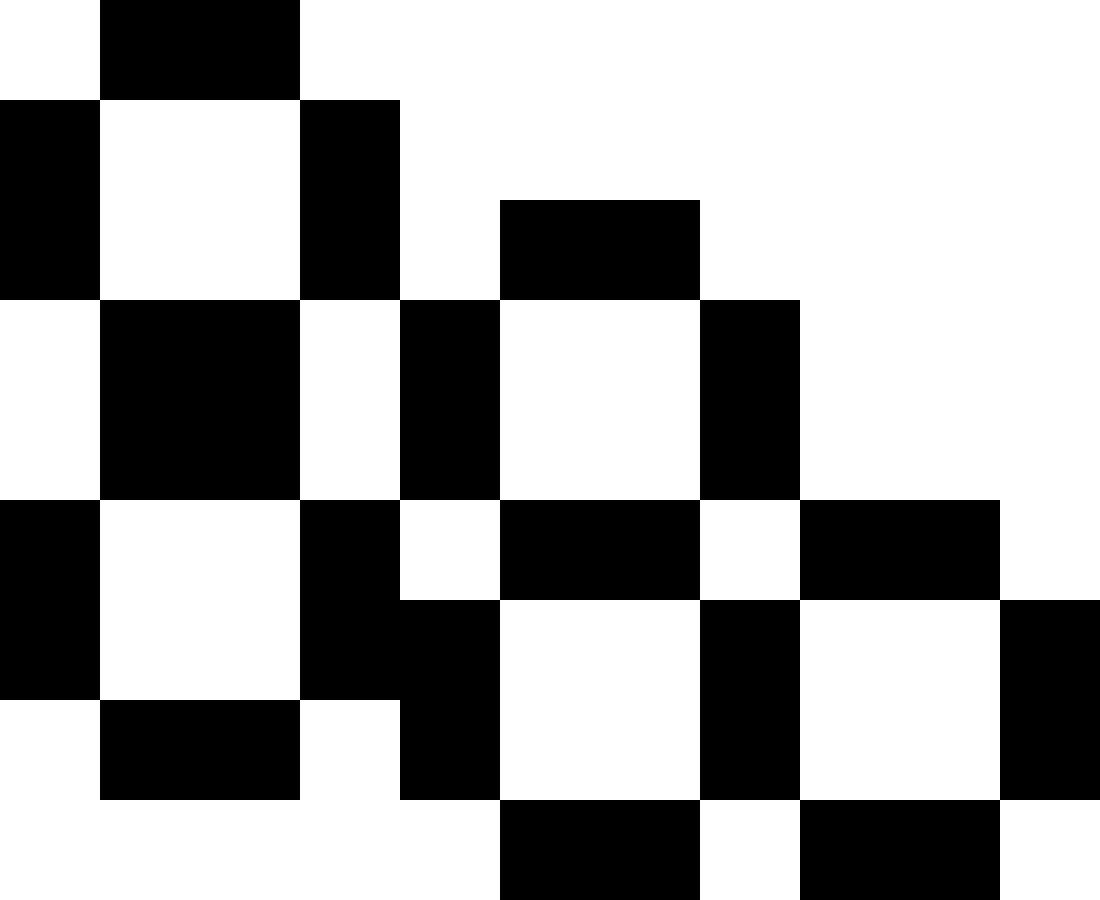
\includegraphics[height=20pt]{Logo}}

\usepackage{float}
\usepackage{listings, color, times, textcomp, float}
\definecolor{mygreen}{RGB}{28,172,0} % color values Red, Green, Blue
\definecolor{mylilas}{RGB}{170,55,241}
\lstset{language=Matlab, basicstyle=\scriptsize\ttfamily,breaklines=true,frame=single,morekeywords={matlab2tikz},
keywordstyle=\color{blue}, morekeywords=[2]{1}, keywordstyle=[2]{\color{black}}, identifierstyle=\color{black},
stringstyle=\color{mylilas}, commentstyle=\color{mygreen}, showstringspaces=false, numbers=left,
numberstyle={\tiny \color{black}}, numbersep=9pt, emph=[1]{for,end,break},emphstyle=[1]\color{red},
literate={~} {\texttildelow}{1}}

\title{MATH 3610 - Project \#1}
\author{Paul Chesnais (pmc85), Christopher Silvia (cps232), Ryan Vogan (rcv39)}
\date{\today}

\newcommand{\exo}[1]{\section*{Exercise #1}}
\newcommand{\prob}[1]{\section*{Problem #1}}
\newcommand{\quest}[1]{\section*{Question #1}}
\newcommand{\e}{&=}
\newcommand{\p}[1]{\times 10^{#1}}
\renewcommand{\headrulewidth}{0pt}
\renewcommand{\footrulewidth}{0.5pt}

\DeclareMathOperator\erf{erf}

\begin{document}
\maketitle
\thispagestyle{fancy}

\section{Decision Variables}

The client has proposed two strategies:

\begin{enumerate}
\item Focus vaccination efforts on the ``most connected''.
\item Focus vaccination efforts on the most frail or susceptible.
\end{enumerate}

In our models, we want to express our choice of policy as a ``decision variable''.
Since we will be recieving 4000 vaccinations a month, our policy recommendation
	will be how to distribute those 4000 vaccinations.
If we identify $n$ categories of Ithacans, each month we will provide 
	recommendations on which fraction of the 4000 vaccines to give to 
	each category of Ithacans.

We should note that each model won't necessarily divide the population into the
	same number of categories.
Each one will provide a different recommendation for the health officials.

\section{Evaluating Models}

Once we chose parameters for our model, we will run it and show its predictions.
We expect that models should at least model the total number of sick
	individuals.
The model might also keep track of how many individuals die.
We have thought of three different ways of evaluating our model:

\begin{enumerate}
\item Total Deaths
\item Total Person-Days Spent Sick
\item Time Until Disease is Eradicated
\end{enumerate}

Note that the models may only provide predictions for some of these criteria.

\section{Simple Continuous Model}

First, we propose a deterministic model which doesn't divide the population 
	into sections at all.
This model will help give us an idea of what the effect of dividing
	the population into sections will be.
In addition, it can give us an idea of how vaccination affects the spread of
	disease within a population.

\subsection{Disease Spread with No Vaccine}

We include this derivation of the logistic model for disease spread
	to compare with our derivation of the modified logistic model
	for disease spread and vaccination.

Suppose there are two groups of people, with $S$ representing the number of 
	sick people, and $H$ represnting the number of healthy people.
Suppose the probability of a single healthy person becoming sick is proportional
	only to the total number of sick people.
Since there are $H$ healthy people, the expected number of healthy people
	who become sick should be proportional to $S H$.
This model does not take into account recovery from sickness.
If we introduce a parameter $r$, we can express this relationship as a system
	of differential equations:

\begin{align*}
\frac{dH}{dt} & = - r S H \\
\frac{dS}{dt} & = r S H \\
\end{align*}

Notice that the total number of people, $S + H$, is conserved, i.e.,

\[ \frac{d}{dt} \left( S + H \right) = \frac{dS}{dt} + \frac{dH}{dt}
	= r S H - r S H = 0 \]

If we introduce another parameter, $K$, to represent the total population,
	such that $S + H = K$ for all time, then the differential equations
	can be decoupled:

\begin{align*}
\frac{dH}{dt} & = - r (K - H) H \\
\frac{dS}{dt} & = r S (K - S) \\
\end{align*}

These are two independant logistic models.

\subsection{Diease Spread with Vaccine}

Suppose we introduce a third group, $V$, representing people who are vaccinated	
	against the disease.
Suppose we randomly vaccinate members of the healthy population,
	a constant number each time step.
This introduces a third parameter, $r_v$, the rate of vaccinations.
The vaccinated population isn't seceptible to the disease.
This process is modeled by the following system of diffential equations:

\begin{align*}
\frac{dS}{dt} & = r S H \\
\frac{dH}{dt} & = - r S H - r_v \\
\frac{dV}{dt} & = r_v
\end{align*}

This model is accurate only if all three of the populations remain
	positive.
This is important to remember.
The number of healthy people will always be decreasing, so once
	the number of healthy people hits zero, we stop the model.
The sick people stay sick, and the vaccinated people stay vaccinated.

The number of vaccinated people as a function of time is:

\[ V(t) = r_v t \]

Again, we find the conserved quantity $\left( S + H + V \right)$ and
	name it $K$.
For the model to be valid, we need $H = K - S - V \geq 0$.
Therefore, the model is valid as long as:

\[ K \geq S + r_v t \]

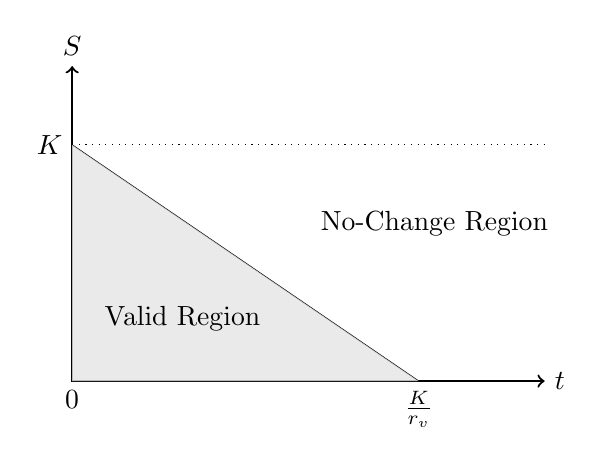
\begin{tikzpicture}[scale=2.0]
	\coordinate[label=below:{$0$}] (origin) at (0,0);
	\draw[<->, thick] (0,2) node (saxis) [above] {$S$}
	|- (3,0) node (taxis) [right] {$t$};
	
	\coordinate[label=left:{$K$}] (sintercept) at (0,1.5);
	\coordinate[label=below:{$\frac{K}{r_v}$}] (tintercept) at (2.2,0);
	\draw (sintercept) -- (tintercept);
	\fill[gray!20, opacity=0.8] (origin) -- (sintercept) -- (tintercept) -- cycle;

	\draw[dotted] (sintercept) -- (3.0, 1.5);
	\node (valid) at (0.7,0.4) {Valid Region};
	\node (endregion) at (2.3, 1.0) {No-Change Region};
\end{tikzpicture}

In the above figure, once $S(t)$ hits the diagonal line,
	it stays horizontal and keeps its value.

We have now made these differential equations independant,
	within the model's zone of validity:

\begin{align*}
\frac{dS}{dt} & = r S \left( K - S - r_v t \right)\\
\frac{dH}{dt} & = - r H \left( K - H - r_v t \right) - r_v \\
\frac{dV}{dt} & = r_v t
\end{align*}

We present a solution for $S(t)$:

\begin{align}
S(t) & = 
	\frac{e^{ r t (K - \frac{ r_v t}{2})}}
	{\frac{1}{S(0)} + \sqrt{\frac{\pi r}{2 r_v}}
		e^{\frac12 \left( \frac{r}{r_v} \right) K^2}
		\left(\erf\left(  \sqrt{\frac{r}{2 r_v}} (r_v t - K ) \right)
			- \erf\left( - \sqrt{\frac{r}{2 r_v}} K \right) \right)}
\end{align}

From the above expression for the boundary of the valid region,
	we get the following implicit expression for $t_f, S(t_f)$

\begin{align}
S(t_f) = 
	\frac{e^{ r t_f (K - \frac{ r_v t_f }{2})}}
	{\frac{1}{S(0)} + \sqrt{\frac{\pi r}{2 r_v}}
		e^{\frac12 \left( \frac{r}{r_v} \right) K^2}
		\left(\erf\left(  \sqrt{\frac{r}{2 r_v}} (r_v t_f - K ) \right)
			- \erf\left( - \sqrt{\frac{r}{2 r_v}} K \right) \right)}
	& = K - r_v t_f 
\end{align}

Here is a family of values of $S(t)$.
The total population and the rate of distributing vaccines are
	held constant, while each curve corresponds to a different
	value of the growth rate constant.
Each curve starts with an initial condition at 5 percent of the
	population, and the growth rate determines how many people
	overall are infected.

\paragraph{}
\pgfplotstableread[col sep = comma]{data/s.csv}\mydata
\begin{tikzpicture}
	\begin{axis}[
		legend pos = south east,
		xmin = 0,
		xmax = 6,
		ymin = 0,
		ymax = 1.3,
		ylabel = {$S(t)$ (units of total population)},
		xlabel = {$t$}
	]
	\foreach \index in {1, ..., 35} {%
		\addplot[mark=""] table[x index = {0}, y index = {\index}]{\mydata};
	}
	\addplot[mark=""] {1 - x * 0.2};
	\end{axis}
\end{tikzpicture}
\paragraph{}

\end{document}
